\documentclass{article}
\usepackage{homework}
\usepackage{amsmath}
\usepackage{amsthm}
\usepackage{listings}
\usepackage{graphicx}
\newcommand{\ea}[1]{\begin{eqnarray*}#1\end{eqnarray*}}
\newcommand{\eanum}[1]{\begin{eqnarray}#1\end{eqnarray}}
\newcommand{\leftbrace}[1]{\left\{\begin{array}{ll}#1 \end{array}\right.}
\newcommand{\norminf}[1]{\left\|{#1}\right\|_\infty}
\newcommand{\twonorm}[1]{\left\|{#1}\right\|_{2}}
\newcommand{\norm}[1]{\left\|{#1}\right\|}
\newcommand{\mat}[2]{\left[\begin{array}{#1}#2\end{array}\right]}
\newcommand{\inv}[1]{#1^{-1}}
\newcommand{\inner}[1]{\left\langle {#1} \right\rangle}
\newcommand{\R}{\mathcal{R}}
\newcommand{\abs}[1]{\vert{#1}\vert}
\author{Roman Stanchak}
\title{Homework 5}
\begin{document}
\bibliographystyle{plain}
\maketitle
%%%%%%%%%%%%%%%%%%%%%%%%%%%%%%%%%%%%%%%%%%%%%%%%%%%%%%%%%%%%%%%%%%%%%%%%%%%%%%%%
%%%%%%%%%%%%%%%%%%%%%%%%%%%%%%%%%%%%%%%%%%%%%%%%%%%%%%%%%%%%%%%%%%%%%%%%%%%%%%%%
%%%%%%%%%%%%%%%%%%%%%%%%%%%%%%%%%%%%%%%%%%%%%%%%%%%%%%%%%%%%%%%%%%%%%%%%%%%%%%%%
\problem{1} If $e^{(0)}=\hat{e}^{(0)}$ and $\rho(S_1) < \rho(S_2)$, is it the 
case that $\norm{ e^{(k)} } < \norm{\hat{e}^{(k)}}$?  If so, prove it, otherwise provide
a counter example.
%%%%%%%%%%%%%%%%%%%%%%%%%%%%%%%%%%%%%%%%%%%%%%%%%%%%%%%%%%%%%%%%%%%%%%%%%%%%%%%%
\solution{1} 
Consider the following values for $A,b,Q_1,Q_2$:
\ea{
A&=& \mat{cc}{2 & 0 \\ 0 & 1}\\
b&=& \mat{c}{1 \\ 1}\\
}
Trivially, the true solution is $x=[\frac{1}{2}, 1]$.  
Consider the following splittings:
\ea{
	Q_1&=& \mat{cc}{20 & 0 \\ 0 & 10}\\
	Q_2&=& \mat{cc}{200 & 0 \\ 0 & 1+\frac{1}{99}}
}
The associated iteration matrices are:
\ea{
	S_1&=& \mat{cc}{.9 & 0 \\ 0 & .9}\\
	S_2&=& \mat{cc}{.99 & 0 \\ 0 & .01}
}
Trivially,
\ea{
	\rho(S_1)&=& .9\\
	\rho(S_2)&=& .99\\
	\rho(S_2) > \rho(S_1)
}
Starting with initial estimate $x^{(0)}=[0 0]$, have $e^{(0)}=[\frac{1}{2}, 1]$.
After applying one iteration:
\ea{
	e^{(1)} &=& \mat{c}{.45 \\ .9}\\
	\hat{e}^{(1)}&=& \mat{c}{.495 \\ .01}\\
	\norm{ e^{(1)} } &\approx& 1.062 \\
	\norm{ \hat{e}^{(1)} } &\approx&  0.49510 
}
Thus, it is not the case that $\norm{ e^{(k)} } < \norm{\hat{e}^{(k)}}$.
%%%%%%%%%%%%%%%%%%%%%%%%%%%%%%%%%%%%%%%%%%%%%%%%%%%%%%%%%%%%%%%%%%%%%%%%%%%%%%%%
%%%%%%%%%%%%%%%%%%%%%%%%%%%%%%%%%%%%%%%%%%%%%%%%%%%%%%%%%%%%%%%%%%%%%%%%%%%%%%%%
%%%%%%%%%%%%%%%%%%%%%%%%%%%%%%%%%%%%%%%%%%%%%%%%%%%%%%%%%%%%%%%%%%%%%%%%%%%%%%%%
\problem{2} Implement Jacobi method, the Gauss-Seidel method, the SOR method and 
the conjugate gradient method.
%%%%%%%%%%%%%%%%%%%%%%%%%%%%%%%%%%%%%%%%%%%%%%%%%%%%%%%%%%%%%%%%%%%%%%%%%%%%%%%%
\solution{2} 
See attached for source code.
As can be seen in Figures\ref{fig:iter} and \ref{fig:time}, as $n$ increases, 
the number of iterations and execution time for Jacobi, GS and SOR seem to increase
on the order of $n^2$.  On the other hand, Conjugate Gradient, and the built-in 
'solve' function seem to increase linearly with $n$.
\begin{figure}[htb]
	\center{
	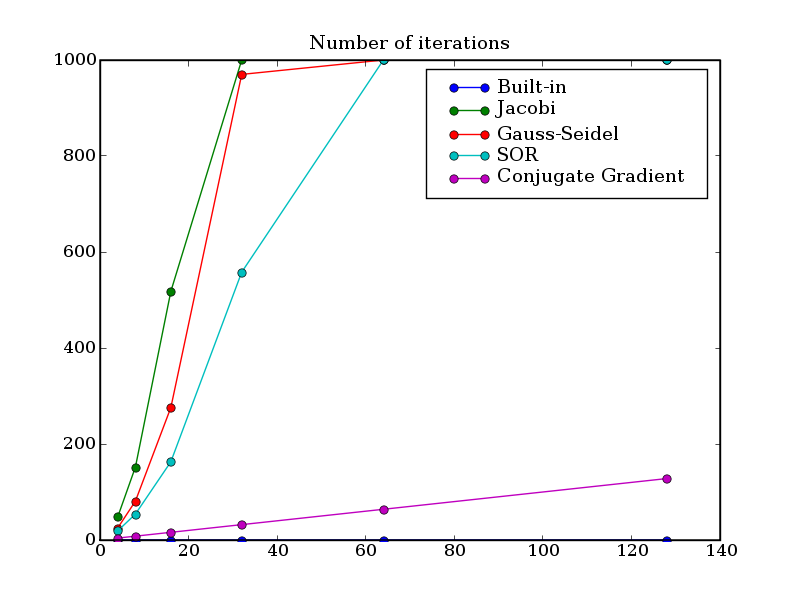
\includegraphics[width=4in]{itersolve_iter}
	\caption{ Number of iterations to convergence (Max is 10000)}
			\label{fig:iter}
	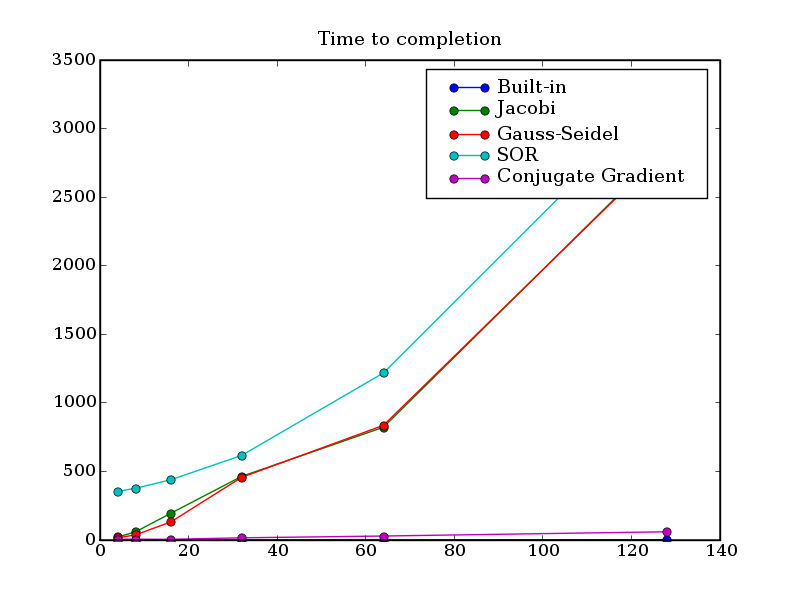
\includegraphics[width=4in]{itersolve_time}
	\caption{ Amount of time until convergence (ms) (Max 10000 iterations)}
			\label{fig:time}
	}
\end{figure}

%%%%%%%%%%%%%%%%%%%%%%%%%%%%%%%%%%%%%%%%%%%%%%%%%%%%%%%%%%%%%%%%%%%%%%%%%%%%%%%%
%%%%%%%%%%%%%%%%%%%%%%%%%%%%%%%%%%%%%%%%%%%%%%%%%%%%%%%%%%%%%%%%%%%%%%%%%%%%%%%%
%%%%%%%%%%%%%%%%%%%%%%%%%%%%%%%%%%%%%%%%%%%%%%%%%%%%%%%%%%%%%%%%%%%%%%%%%%%%%%%%
\problem{3a} Show that the Chebyshev polynomials $\tau_k(t)$ satisfy the three
term recurrence:
\[
	\tau_{k+1}(t) = 2t\tau_k(t) - \tau_{k-1}(t)
\]
%%%%%%%%%%%%%%%%%%%%%%%%%%%%%%%%%%%%%%%%%%%%%%%%%%%%%%%%%%%%%%%%%%%%%%%%%%%%%%%%
\solution{3a} 
Proof by Induction on $k$.\\
\begin{proof}[Proof of Base Cases, $k=0,1,2; t\le \abs{1}$]
\ea{
	T_0(t) &=& 1\\
	T_1(t) &=& \cos \inv{\cos} t \\
		   &=& t \\
	T_2(t) &=& \cos 2\inv{\cos} t \\ 
	\textrm{let:}\\
	\theta &=& \inv{\cos} t \\
	T_2(\theta) &=& \cos 2 \theta \\
	 	   &=& 2 \cos^2 \theta - 1 \\
		   &=& 2 t^2 - 1\\
	T_2(t) &=& 2 t \cdot T_1(t) - T_0(t)
}
\end{proof}
\begin{proof}[Inductive Case]
	Assume true for all $j\le k$, prove for $k+1$.
\ea{
T_{k+1} &=& \cos \left( (k+1) \inv{\cos}(t) \right)\\
	&=& \cos (k+1)\theta \\
	&=& \cos k\theta\cos\theta - \sin k\theta\sin\theta \\
	&=& t\cdot\cos k\theta - \sin k\theta\sin\theta \\
	&=& t\cdot T_k(t) - \sin k\theta\sin\theta \\
	&=& t\cdot T_k(t) - \frac{1}{2}\left[\cos( k\theta - \theta ) - \cos( k\theta + \theta ) \right] \\
	&=&  t\cdot T_k(t) - \frac{1}{2}T_{k-1}(t) + \frac{1}{2}T_{k+1}(t) \\
	\frac{1}{2} T_{k+1}(t) &=& t\cdot T_k(t) - \frac{1}{2}T_{k-1}(t) \\
	T_{k+1}(t) &=&  2t\cdot T_k(t) - T_{k-1}(t)
}
\end{proof}
When $t > |1|$:
	\textit{ see attached }
%%%%%%%%%%%%%%%%%%%%%%%%%%%%%%%%%%%%%%%%%%%%%%%%%%%%%%%%%%%%%%%%%%%%%%%%%%%%%%%%
%%%%%%%%%%%%%%%%%%%%%%%%%%%%%%%%%%%%%%%%%%%%%%%%%%%%%%%%%%%%%%%%%%%%%%%%%%%%%%%%
%%%%%%%%%%%%%%%%%%%%%%%%%%%%%%%%%%%%%%%%%%%%%%%%%%%%%%%%%%%%%%%%%%%%%%%%%%%%%%%%
\problem{3b} Prove that:
\[
	\tau_k(t) = \frac{1}{2}\left[ \left(t+\sqrt{t^2-1}\right)^k + 
		\left(t-\sqrt{t^2-1}\right)^k\right]
\]
%%%%%%%%%%%%%%%%%%%%%%%%%%%%%%%%%%%%%%%%%%%%%%%%%%%%%%%%%%%%%%%%%%%%%%%%%%%%%%%%
\solution{3b}
\ea{
\tau_k(t) &=& \cos k \inv{\cos t}\\
	&=& \frac{1}{2}e^{ik\inv{\cos t}} + \frac{1}{2}e^{-ik\inv{\cos t}} \\
	\inv{\cos t} &=& -i \textrm{ln}(t + i\sqrt{1-t^2})\\
	&=& \frac{1}{2}e^{ik(-i \textrm{ln}(t + i\sqrt{1-t^2}))} + 
		\frac{1}{2}e^{-ik(-i \textrm{ln}(t + i\sqrt{1-t^2}))} \\
		&=&  \frac{1}{2}e^{k\textrm{ln}(t+i\sqrt{1-t^2})} +
		\frac{1}{2}e^{-k\textrm{ln}(t+i\sqrt{1-t^2})} \\
		&=&  \frac{1}{2}e^{\textrm{ln}(t+i\sqrt{1-t^2})^k} + 
		\frac{1}{2}e^{\textrm{ln}(t+i\sqrt{1-t^2})^{-k}} \\
	&=& \frac{\left( t + i \sqrt{1-t^2} \right)^k }{2} +
		\frac{1}{2\left( t + i \sqrt{1-t^2} \right)^k} \\
		&=& \frac{\left( t + i \sqrt{1-t^2} \right)^{2k} + 1}
	        {2\left( t + i \sqrt{1-t^2} \right)^k}
}
Proof by induction on $k$
\begin{proof}[Base case, $k=1$]
\ea{
	\tau_1(t) &=&  \frac{\left( t + i \sqrt{1-t^2} \right)^{2} + 1}
	            {2\left( t + i \sqrt{1-t^2} \right)}\\
			&=& \frac{ t^2 + 2it\sqrt{1-t^2} - (1-t^2) + 1}
				{2\left( t + i \sqrt{1-t^2} \right)}\\
			&=& \frac{ 2t^2 + 2it\sqrt{1-t^2} + 0}
				 {2\left( t + i \sqrt{1-t^2} \right)}\\
			&=& t \\
			&=& \frac{1}{2}(t + \sqrt{t^2-1}) + \frac{1}{2}(t - \sqrt{t^2-1})
}
\end{proof}
\begin{proof}[Inductive case, assume for $j\le k$, prove for $k+1$]
\ea{
	\tau_{k+1}(t) &=&  2t\cdot\tau_k(t) - \tau_{k-1}(t) \\
	&=& \frac{1}{2}\left[ \left(t+\sqrt{t^2-1}\right)^k + \left(t-\sqrt{t^2-1}\right)^k\right]\cdot 2t -
	\frac{1}{2}\left[ \left(t+\sqrt{t^2-1}\right)^{k-1} + \left(t-\sqrt{t^2-1}\right)^{k-1}\right] \\
	&=& \frac{1}{2}\left[ \left(t+\sqrt{t^2-1}\right)^{k-1}\left[\left(t+\sqrt{t^2-1}\right)\cdot 2t - 1\right] +
	                      \left(t-\sqrt{t^2-1}\right)^{k-1}\left[\left(t-\sqrt{t^2-1}\right)\cdot 2t - 1\right] \right] \\
	&=& \frac{1}{2}\left[ \left(t+\sqrt{t^2-1}\right)^{k-1}\left[2t^2 + 2t\sqrt{t^2-1} -1\right] +
	                       \left(t-\sqrt{t^2-1}\right)^{k-1}\left[2t^2 - 2t\sqrt{t^2-1} -1\right] \right] 
}
Note that:
\ea{
(t+\sqrt{t^2-1})^2 &=& t^2+2t\sqrt{t^2-1} + t^2 -1 \\
											&=& 2t^2+2t\sqrt{t^2-1} -1 
}
And:
\ea{
	(t-\sqrt{t^2-1})^2 &=& t^2-2t\sqrt{t^2-1} + t^2 -1 \\
								     &=& 2t^2-2t\sqrt{t^2-1} -1 
}
So:
\ea{
	\tau_{k+1}(t) &=& \frac{1}{2}\left[ \left(t+\sqrt{t^2-1}\right)^{k-1}(t+\sqrt{t^2-1})^2 + 
										\left(t-\sqrt{t^2-1}\right)^{k-1}(t-\sqrt{t^2-1})^2 \right] \\
				&=& \frac{1}{2}\left[ \left(t+\sqrt{t^2-1}\right)^{k+1} + 
				        \left(t-\sqrt{t^2-1}\right)^{k+1}\right]
}
\end{proof}
%%%%%%%%%%%%%%%%%%%%%%%%%%%%%%%%%%%%%%%%%%%%%%%%%%%%%%%%%%%%%%%%%%%%%%%%%%%%%%%%
%%%%%%%%%%%%%%%%%%%%%%%%%%%%%%%%%%%%%%%%%%%%%%%%%%%%%%%%%%%%%%%%%%%%%%%%%%%%%%%%
%%%%%%%%%%%%%%%%%%%%%%%%%%%%%%%%%%%%%%%%%%%%%%%%%%%%%%%%%%%%%%%%%%%%%%%%%%%%%%%%
\problem{4a} Given a symmetric positive-definite matrix $A$ of order $n$, show that
$\inner{x,y}_A$  defines an inner product on $\R_n$.

%%%%%%%%%%%%%%%%%%%%%%%%%%%%%%%%%%%%%%%%%%%%%%%%%%%%%%%%%%%%%%%%%%%%%%%%%%%%%%%%
\solution{4a} 
Show $\inner{x,y}_A = \inner{y,x}_A$.
\begin{proof}
	\ea{
		\inner{x,y}_A &=& (x,Ay) \\
				&=& x^TAy \\
				&=& x^TA^Ty \\
				&=& y^TAx \\
				&=& \inner{y,x}
	}
\end{proof} 
Show $\inner{\alpha x, y}_A = \alpha\inner{x,y}_A$.
\begin{proof}
	\ea{
		\inner{\alpha x,y}_A &=& (x, \alpha Ay) \\
			&=& \alpha(x,Ay) \\
			&=& \alpha\inner{x,y}_A
	}
\end{proof}
Show $\inner{x+z,y}_A = \inner{x,y}_A + \inner{z,y}_A$
\begin{proof}
	\ea{
		\inner{x+z,y}_A &=& \inner{y,x+z}_A\\
			&=& (y, A(x+z))\\
			&=& (y, Ax+Az)\\
			&=& (y,Ax) + (y,Az) \\
			&=& \inner{y,x}_A + \inner{y,z}_A \\
			&=& \inner{x,y}_A + \inner{z,y}_A
	}
\end{proof}
Show $\inner{x,x}_A \ge 0,\textrm{  }0 \iff x=0$
\begin{proof}
\ea{
	\inner{x,x}_A &=& (x, Ax) = x^TAx \\
	x^TAx > 0 &\iff& x>0  \textrm{    By definition of positive definite}\\
	\implies \\
	\inner{x,x}_A \ge 0, && = 0 \iff x=0
}
\end{proof}
%%%%%%%%%%%%%%%%%%%%%%%%%%%%%%%%%%%%%%%%%%%%%%%%%%%%%%%%%%%%%%%%%%%%%%%%%%%%%%%%
%%%%%%%%%%%%%%%%%%%%%%%%%%%%%%%%%%%%%%%%%%%%%%%%%%%%%%%%%%%%%%%%%%%%%%%%%%%%%%%%
%%%%%%%%%%%%%%%%%%%%%%%%%%%%%%%%%%%%%%%%%%%%%%%%%%%%%%%%%%%%%%%%%%%%%%%%%%%%%%%%
\problem{4b} A matrix $B$ is symmetric with respect to an inner product 
$\inner{·, ·}$ if  $\inner{Bx, y} = \inner{x, By}$. Show that if $A$ and $Q$ are 
symmetric positive-definite, then $\inv{Q}A$ is symmetric with respect to the 
inner product $\inner{·, ·}_Q$ .

%%%%%%%%%%%%%%%%%%%%%%%%%%%%%%%%%%%%%%%%%%%%%%%%%%%%%%%%%%%%%%%%%%%%%%%%%%%%%%%%
\solution{4b} 
\begin{proof}
	\ea{
		\inner{\inv{Q}Ax,y}_Q &=&  (Q\inv{Q}Ax, y) \\
			&=& (x,Ay) \\
			&=&  x^TA^Ty \\
			&=& x^TQ^TQ^{-T}A^Ty \\
			&=& x^TQ^TQ^{-1}Ay \\
			&=& (Qx, \inv{Q}Ay) \\
			&=& \inner{ x, \inv{Q}Ay}
		}
\end{proof}
%%%%%%%%%%%%%%%%%%%%%%%%%%%%%%%%%%%%%%%%%%%%%%%%%%%%%%%%%%%%%%%%%%%%%%%%%%%%%%%%
%%%%%%%%%%%%%%%%%%%%%%%%%%%%%%%%%%%%%%%%%%%%%%%%%%%%%%%%%%%%%%%%%%%%%%%%%%%%%%%%
%%%%%%%%%%%%%%%%%%%%%%%%%%%%%%%%%%%%%%%%%%%%%%%%%%%%%%%%%%%%%%%%%%%%%%%%%%%%%%%%
\problem{5a}Show that
\[              AR_k = R_k S_k - \frac{1}{\alpha_k}[0, \dots , 0, r_k ].   \]
where
\[ S_k = \textit{tridiag}\left[ -\frac{1}{\alpha_{j-1}}, 
                                -\frac{1}{\alpha_j} + \frac{\beta_{j-1}}{\alpha_{j-1}},
								-\frac{\beta_j}{\alpha_j} \right]
\]
%%%%%%%%%%%%%%%%%%%%%%%%%%%%%%%%%%%%%%%%%%%%%%%%%%%%%%%%%%%%%%%%%%%%%%%%%%%%%%%%
\solution{5a} The step to update the residual $r$ goes as follows:
\[ r^{(j+1)} = r^{(j)} - \alpha_j A p^{(j)} \]
The step to update the 'update' vector $p$:
\[ p^{(j)} = r^{(j)} + \beta_j p^{(j-1)} \]
Substituting $p^{(j)}$:
\[ r^{(j+1)} = r^{(j)} - \alpha_j A  r^{(j)} - \alpha_j\beta_j A p^{(j-1)} \]
Rewriting the residual step for $j$:
\[ A p^{(j-1)} = \frac{ r^{(j-1)} - r^{(j)} }{\alpha_{j-1}} \]
And plugging back in above for $A p^{(j-1)}$:
\[  r^{(j+1)} = r^{(j)} - \alpha_j A  r^{(j)} - \frac{\alpha_j\beta_j}{\alpha_{j-1}} \left( r^{(j-1)} - r^{(j)} \right) \]
Rearranging terms:
\[ A r^{(j)} = \frac{1}{\alpha_j}(r^{(j)} - r^{(j+1)}) - \frac{\beta_j}{\alpha_{j-1}}  \left( r^{(j-1)} - r^{(j)} \right) \]
For $j=0,1\dots k-1$:

\ea{
	A r^{(0)} &=& \frac{1}{\alpha_0}(r^{(0)} - r^{(1)}) \\
	A r^{(1)} &=&  \frac{1}{\alpha_1}(r^{(1)} - r^{(2)}) - \frac{\beta_1}{\alpha_{0}}  \left( r^{(0)} - r^{(1)} \right) \\
	A r^{(2)} &=&  \frac{1}{\alpha_2}(r^{(2)} - r^{(3)}) - \frac{\beta_2}{\alpha_{1}}  \left( r^{(1)} - r^{(2)} \right) \\
	\dots\\
	A r^{(k-1)} &=&  \frac{1}{\alpha_{k-1}}(r^{(k-1)} - r^{(k)}) - \frac{\beta_{k-1}}{\alpha_{k-2}}  \left( r^{(k-2)} - r^{(k-1)} \right)
}
Collecting the common coefficients in $r^{(0)}\dots r^{(k-1)}$ this forms the linear system:
\[ A [r^{(0)}, r^{(1)} \dots r^{(k-1)}] = [r^{(0)}, r^{(1)} \dots r^{(k-1)}] 
	\mat{ccccc}{ \frac{1}{\alpha_0} & - \frac{\beta_1}{\alpha_{0}} & 0 & \dots & 0 \\
	-\frac{1}{\alpha_0} & \frac{1}{\alpha_1} + \frac{\beta_1}{\alpha_0} &  - \frac{\beta_2}{\alpha_{1}} & 0 & \dots  \\
	\dots \\
	\dots \\
	0 & \dots & 0 & -\frac{1}{\alpha_{k-2}} & \frac{1}{\alpha_{k-1}} + \frac{\beta_{k-1}}{\alpha_{k-2}} 
	} + \frac{1}{\alpha_{k-1}}r^{(k)}\mathbf{e}^{(k)}
\]
Where $\mathbf{e}^{(k)}$ is the $k+1$th column of the identity matrix.  \\
This is exactly the form desired:
\[              AR_k = R_k S_k - \frac{1}{\alpha_k}[0, \dots , 0, r_k ].   \]
%%%%%%%%%%%%%%%%%%%%%%%%%%%%%%%%%%%%%%%%%%%%%%%%%%%%%%%%%%%%%%%%%%%%%%%%%%%%%%%%
%%%%%%%%%%%%%%%%%%%%%%%%%%%%%%%%%%%%%%%%%%%%%%%%%%%%%%%%%%%%%%%%%%%%%%%%%%%%%%%%
%%%%%%%%%%%%%%%%%%%%%%%%%%%%%%%%%%%%%%%%%%%%%%%%%%%%%%%%%%%%%%%%%%%%%%%%%%%%%%%%
\problem{5b} Show that $S_k$ is similar to a symmetric matrix $T_k$ . Where 
have you seen the matrix $T_k$ before?
%%%%%%%%%%%%%%%%%%%%%%%%%%%%%%%%%%%%%%%%%%%%%%%%%%%%%%%%%%%%%%%%%%%%%%%%%%%%%%%%
\solution{5b} 
Need to show that there exists an invertible $k\times k$ matrix $U$ s.t.
\[ US_k\inv{U} = T_k \]
or perhaps that $S_k$ and $T_k$ have the same eigenvalues.  $T_k$ is most likely
the matrix of coefficients from the Lanczos procedure, but $\alpha$ and $\beta$
are probably different.  I'm fairly certain that if $v^{(1)}=x^{(0)}$, both the set 
of $\{r^{(j)}\}$ and the Lanczos basis vectors $\{v^{(j)}\}$ span the Krylov 
subspace $K(A,x^{(0)}$, but I'm not sure how this helps.  
%%%%%%%%%%%%%%%%%%%%%%%%%%%%%%%%%%%%%%%%%%%%%%%%%%%%%%%%%%%%%%%%%%%%%%%%%%%%%%%%
%%%%%%%%%%%%%%%%%%%%%%%%%%%%%%%%%%%%%%%%%%%%%%%%%%%%%%%%%%%%%%%%%%%%%%%%%%%%%%%%
%%%%%%%%%%%%%%%%%%%%%%%%%%%%%%%%%%%%%%%%%%%%%%%%%%%%%%%%%%%%%%%%%%%%%%%%%%%%%%%%
\problem{6} Show the PCG algorithm can be interpreted as an implementation of
solving the normal CG on the following system:
\[
\left[\inv{L} AL^T \right]\hat{x} = \left[\inv{L}b\right]
\]
where $Q=LL^T$ and $\hat{x}=L^{-T}x$.
%%%%%%%%%%%%%%%%%%%%%%%%%%%%%%%%%%%%%%%%%%%%%%%%%%%%%%%%%%%%%%%%%%%%%%%%%%%%%%%%
\solution{6} The PCG algorithm proceeds as follows:
\ea{
x^{(0)} &=& \textit{arbitrary} \\
r^{(0)} &=& b - Ax^{(0)} \\
\tilde{r}^{(0)} &=& Q\left( b-Ax^{(0)} \right) \\
p^{(0)} &=& \tilde{r}^{(0)} \\
x^{(j+1)} &=& x^{(j)} + \alpha_j p^{(j)} \\
r^{(j+1)} &=& r^{(j)} + \alpha_j Ap^{(j)} \\
\tilde{r}^{(j+1)} &=& Qr^{(j+1)} \\
\beta_j &=& ?? \\
p^{(j+1)} &=& \tilde{r}^{(j)} + \beta_jp^{(j)}
}
TODO: Finish this.
%%%%%%%%%%%%%%%%%%%%%%%%%%%%%%%%%%%%%%%%%%%%%%%%%%%%%%%%%%%%%%%%%%%%%%%%%%%%%%%%
%%%%%%%%%%%%%%%%%%%%%%%%%%%%%%%%%%%%%%%%%%%%%%%%%%%%%%%%%%%%%%%%%%%%%%%%%%%%%%%%
%%%%%%%%%%%%%%%%%%%%%%%%%%%%%%%%%%%%%%%%%%%%%%%%%%%%%%%%%%%%%%%%%%%%%%%%%%%%%%%%
\end{document}
